\documentclass{article}
\usepackage[utf8]{inputenc}
\usepackage{amsmath}
\usepackage{amsfonts}
\usepackage{enumitem}
\usepackage{amssymb} 
\usepackage{xcolor}
\usepackage{soul}
\usepackage{todonotes}
\usepackage[margin=2.5cm]{geometry}
\graphicspath{ {./images/} }

\title{Augmented Data Structure}
\author{Jin Long Cao}
\date{November 2022}

\begin{document}
\maketitle
\noindent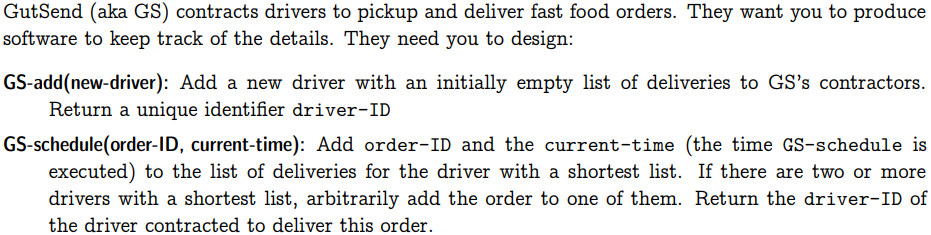
\includegraphics[width=\textwidth]{Augmented Data Structure1}
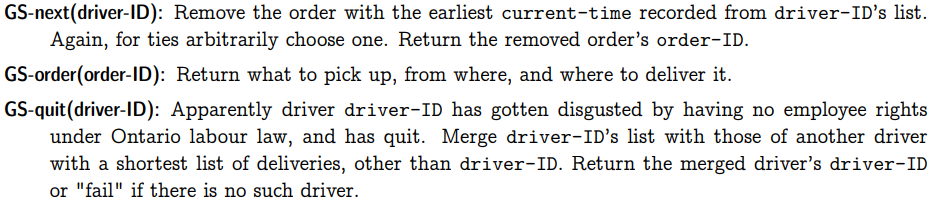
\includegraphics[width=\textwidth]{Augmented Data Structure2}
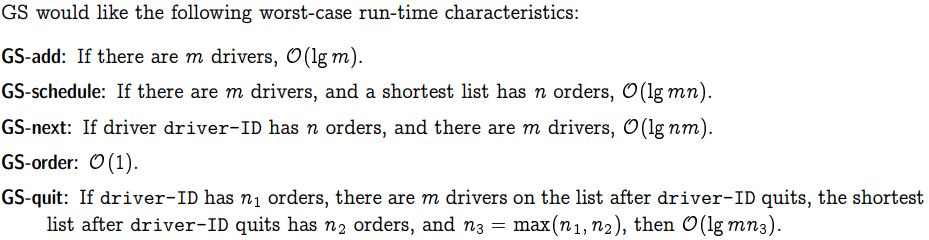
\includegraphics[width=\textwidth]{Augmented Data Structure3}
\section*{Solutions}
% Essentially the goal is the implement these functions such that they have the following worst-case runtime:
% \begin{itemize}
%     \item GS-add: If there are m drivers, \textbf{O(lg m)}. (idea: implement it as a BST to get O(lg m))
%     \item GS-schedule: If there are m drivers, and a shortest list has n orders, \textbf{O(lg mn)}.
%     \item GS-next: If driver driver-ID has n orders, \textbf{O(lg n)}.
%     \item GS-order: \textbf{O(1)} (idea: since it's just returning info, it should just be O(1))
%     \item GS-quit: If driver-ID has n1 orders, there are m drivers on the list after driver-ID quits, the shortest list after driver-ID quits has n2 orders, and n3 = max(n1; n2), then \textbf{O(lg mn3)}.
% \end{itemize}

% GS-quit: 1) Find the driver with driver-ID \\
% 2) Save the driver's list (A)\\
% 3) Find the driver with the shortest list; *need to keep track of list size in driver's satellite value*\\
% 4) Get this driver's list (B)\\
% 5) Merge A and B\\
% Want lg(m) + lg($n_3$)\\
% lg(m) would be step 1, looping through m drivers to find the driver\\
% lg($n_3$) would be step 5? merging?\\
% So delivery must be binomial heap



% \noindent Notes: WORST CASE RUNTIME FOR HASH IS O(n) so hashing will prob not work for this question\\
% GS-add(new-driver):\\
% Create a node — O(1)\\
% How to generate unique driver-ID? Random function? \\
% Create an empty tree for deliveries; assign to driver’s satellite value\\
% Define a satellite value to keep track of the size of the delivery tree; initiate to be 0\\
% Place this new node in the right place in the BST — O(lg(m))	
% \\~\\
% GS-schedule(order-ID, current-time):\\
% Loop through the tree of drivers to find the one with the 			shortest list; since we can access the size of the delivery tree using a satellite value, we don’t have to loop through elements of each delivery tree to count — O(lg(m))\\
% Add order-ID and current-time to the delivery tree — O(lg(n))\\
% Order-ID could be the node value and current-time could be a satellite value\\
% Update the size of the delivery tree; driver.dtreesize += 1 — O(1)\\
% Altogether, O(lg(mn))
% \\~\\
% GS-next(driver-ID):\\
% We already know the driver ID, so we can go directly into the driver tree and find this node. Since there are m drivers, this will take O(lg(m)). We go into the driver’s delivery tree.\\
% 2 steps: finding the order with the earliest current-time (requires looping through the delivery tree node by node and access each node’s satellite value), remove the node\\
% **Problem** Finding the driver from the driver tree takes O(lg(m)), finding the order from the delivery tree takes O(lg(n)), removing the order takes O(lg(n)). This exceeds O(lg(n)) which is what we need.
% \\~\\
% GS-order(order-ID):\\
% Given the order ID, we want to get the node in the delivery tree right away within O(1). \\
% **Problem** But normally search takes WC O(lg(n)). Same problem as driver ID. This prompts us to find a way to look up the key of a node in a faster way, e.g. maybe use a hash table. But hash tables have an average time complexity of O(1), at extreme cases, WC can be O(lg(n)).
% \\~\\
% Current idea: \\
% make drivers a tree (need to decide heap or AVL or what kind) and within that we make a dictionary ADT (dictionaries are often implemented as hash tables)



% \subsection*{GS-add(root, new-driver):}
% \begin{enumerate}[itemsep=0pt,parsep=0pt]
%     \item if root is NIL:  
%     \item \qquad \# Found insertion point: create new node with empty children.
%     \item \qquad root = TreeNode(new-driver)
%     \item \qquad root.list = [] \#implement empty list
%     \item elif new-driver.key $\leq$ root.item.key:
%     \item \qquad root.left = GS-add(root.left, new-driver)
%     \item elif new-driver.key $>$ root.item.key:
%     \item \qquad root.right = GS-add(root.right, new-driver)
%     \item return root
% \end{enumerate}

\subsection*{GS-add(new-driver):} 
We'll implement this using a Priority Queue ADT ($P_1$) with heap size, heap shape, and min-heap order. We'll also have a counter variable (starting at 1) such that it every time we add a new driver, this number increases by 1. When we get a new driver, we'll increase heap size by 1, the counter value will be the new-driver's driver-ID, and increment the counter. Since the counter is increasing, min-heap order will be maintained (cost $O(1)$). 
% , swap with it's parents until min-heap order is restored (if needed), which cost $O(\lg m)$ (for heap size of m). 
Also we'll set a satellite value (driver-ID.list) which will be the initial empty list of deliveries (which cost $O(1)$). For later conveniences, we'll also add another satellite value (driver-ID.size) which will tell us the size of the list (initially set to 0). We'll insert this driver-ID.size into another Priority Queue ADT ($P_2$) with heap size, heap shape, and max-heap order. The node has a variable that keeps track of the driver-ID. Finally, return the unique identifier driver-ID.
% We'll insert this driver-ID into a modified binary search tree \textbf{(bst doesn't work, O(n))} where driver-ID.size is the key (x.key). Inserting in this binary search tree will cost $O(\lg m)$ (for m drivers).

\subsection*{GS-schedule(order-ID, current-time):} 
\textbf{recall}: $\lg (mn) = \lg (m) + \lg (n) \Rightarrow O(\lg m) + O(\lg n) = O(\lg m + \lg n) = O(\lg mn) $\\
For worst-case run-time, it cost $O(\lg n)$ at most to extract minimum from $P_2$ (which gives us driver-ID of the driver with the shortest list of $n$ orders). \\
$O(\lg m)$ to find driver with a shortest list out of whole driver tree ($P_1$).
% to increment driver-ID.size, heapify $P_2$, and add Order-ID ($O(\lg n)$). \\
Current-time will be a satellite value for order-ID and order-ID is in a list of other order-ID in driver-ID.list. \\
Then, we'll add order-ID and order-ID.current-time to driver-ID.list to the driver with the shortest list, increment driver-ID.size.
For later conveniences, we'll insert order-ID.current-time into another Priority Queue ADT ($P_3$) in ascending order where the latest order-ID.current-time has the highest priority. The node has a variable that keeps track of the order-ID. Which takes no more than $O(\lg n)$ (for $n$ orders). \\
Also every time we schedule an order, we'll insert the order's information into a dynamic array (called order) which only cost a constant (e.g. order-ID 3 picks up clothes, from Walmart, and delivers to 123 random street. Then order[3] = "picks up clothes, from Walmart, and delivers to 123 random street."). In general, order[order-ID] = Description of order-ID, what to pick up, from where, and where to deliver it. Two orders should not have the same order-ID, if it does, the newer one replaces the later one.\\
Hence, if there are $m$ drivers, and a shortest list of $n$ orders then it would take $O(\lg n)$ to find the driver with the shortest list and it will take $O(\lg m)$ to find such driver.
\begin{align*}
    O(\lg m) + O(\lg n) &= O(\lg m + \lg n) \\
    &= O(\lg mn) 
\end{align*}
It will take $O(\lg mn)$ to satisfies such task. Finally, return the driver-ID of the driver contacted to deliver such order.
% \textbf{Goal:} to find the driver with the shortest list (which has n orders) in $O(\lg n)$ (tree?).\\
% thoughts: driver-ID.list is in a tree but what will it cost to put it in a tree?

\subsection*{GS-next(driver-ID):} 
It costs $O(\lg m)$ to find driver-ID out of all the drivers from $P_1$ (where there are $m$ drivers).\\
Now, we want to find the order-ID with the earliest current-time recorded (out of $n$ orders) in $O(\lg n)$. This can be done my extracting minimum element from $P_3$ which takes at most $O(\lg n)$.\\
Hence, if driver driver-ID has $n$ orders, and there are $m$ drivers, then it would take $\lg m$ to find the specific driver and $\lg n$ to find the order-ID of the specific driver's earliest order-ID. Since the order-ID is found, removing and returning the removed order's order-ID will only take a constant. 
\begin{align*}
    O(\lg n) + O(\lg m) &= O(\lg n + \lg m) \\
    &= O(\lg mn) 
\end{align*}
It will take $O(\lg mn)$ to satisfies such task. Finally, return the removed order's order-ID.

\subsection*{GS-order(order-ID):} 
In GS-schedule, every time we scheduled something, the order's information has been added to a dynamic array (called order). Just like an normal java or python list/array, to insertion and searching in an array cost $O(1)$. It's like setting a variable to something. No matter how big the array is or how many drivers there is, it will always cost $O(1)$ to search for the information of an order-ID. Return order[order-ID] to return what to pick up, from where, and where to deliver it of order's order-ID. 

\subsection*{GS-quit(driver-ID):} 
There's two cases that could happen,
\begin{enumerate}
    \item If shortest list is the driver that quits (such that $n_1 \leq n_2$) then $n_3 = n_2$ and the worst-case run-time cost $O(\lg n_2) = O(\lg n_3)$ at most to extract minimum from $P_2$ (which gives us driver-ID of the driver with the shortest list of $n_2$ orders)
    \item If the shortest list is not the driver that quits (such that $n_1 \geq n_2$) then $n_3 = n_1$ and the worst-case run-time cost $O(\lg n_1) = O(\lg n_3)$ at most to extract minimum from $P_2$ (which gives us driver-ID of the driver with the shortest list of $n_2$ orders)
\end{enumerate}
Notice that in any case it takes $O(\lg n_3)$ to find the driver with the shortest list and $O(\lg m)$ to find driver with a shortest list out of whole driver tree ($P_1$).\\
Hence, if driver-ID has $n_1$ orders, there are $m$ drivers on the list after driver-ID quits, the shortest list after driver-ID quits has $n_2$ orders, and $n_3 = $ max$(n_1,n_2)$, then
\begin{align*}
    O(\lg \text{max}(n_1,n_2)) + O(\lg m) &= O(\lg n_3) + O(\lg m) \\
    &= O(\lg mn_3)
\end{align*}
It will take $O(\lg mn_3)$ to satisfies such task. Finally, return the merged driver's driver-ID.
\end{document}